\documentclass[11pt]{article}
\usepackage[a4paper,margin=1in]{geometry}
\usepackage{amsmath,amssymb,amsthm,mathtools}
\usepackage{booktabs}
\usepackage{enumitem}
\usepackage{graphicx}
\usepackage{hyperref}
\usepackage[nameinlink,capitalise]{cleveref}
\usepackage[numbers,sort&compress]{natbib}

\newtheorem{theorem}{Theorem}[section]
\newtheorem{proposition}[theorem]{Proposition}
\newtheorem{corollary}[theorem]{Corollary}
\theoremstyle{remark}
\newtheorem{remark}[theorem]{Remark}
\newcommand{\norm}[1]{\left\lVert#1\right\rVert}
\newcommand{\cR}{\mathcal R}

\title{Optimal Endpoint Singular Factorization and the Coordinate-Matching Barrier\\
\large Majorization, Dynamical Outer Maps, and the Next All-Level Gate}
\author{Liang Wang}
\date{July 2026}

\begin{document}
\maketitle

\begin{abstract}
RH-82 reduced the preferred Stage-A route to a factorization of the physical
postblock state through the endpoint Gaussian resolution operator.  This
paper determines exactly what such a factorization requires and rules out an
overly literal coordinate realization.

Let $\cR$ have singular values $\rho_1\ge\rho_2\ge\cdots>0$, and let a
rank-$r$ target $B_r$ have singular values $b_1\ge\cdots\ge b_r>0$.  We prove
the optimal two-sided factorization formula
\[
 \inf_{B_r=U\cR V}\norm U\norm V
 =\max_{1\le j\le r}\frac{b_j}{\rho_j}.
\]
The lower bound is the ideal property of approximation numbers; equality is
attained by aligning the two singular systems.  For an arbitrary compact
$B$, its truncated SVD therefore gives
\[
 B=U\cR V+E_r,
 \qquad \norm{E_r}_2=\tau_r(B).
\]
Consequently, singular-value majorization is sufficient for the RH-82
endpoint-to-postblock criterion.  No coordinate alignment of singular vectors
is needed.

A 192-bit audit compares the RH-16 linear endpoint Gram operator with all ten
RH-77 frozen postblock states.  At ranks within one of
$\lceil H_\sigma\rceil+2$, the optimal factor constant is at most $0.161572$
and the largest Hilbert--Schmidt remainder is $1.232\times10^{-9}$.  The
largest relative remainder is $2.340\times10^{-7}$.

By contrast, direct coordinate projection onto sampled endpoint-row vectors
leaves between $46.86\%$ and $97.90\%$ relative residual.  Thus the identity
outer map is decisively unsupported.  The endpoint mechanism can survive only
through a nontrivial dynamical rotation or, equivalently, an all-level
singular-value majorization theorem.

The latter theorem remains open, so uniform Stage A1 and unconditional Stage
A4 are not claimed.  No Hilbert--Polya or Riemann-hypothesis conclusion is
made.
\end{abstract}

\noindent\textbf{Keywords:} singular-value majorization; operator
factorization; endpoint resolution; approximation numbers; effective rank.

\medskip
\noindent\textbf{MSC 2020:} 47A68; 47B06; 47B10; 65G20.

\section{Why the outer maps matter}

RH-82 proved exponential Hilbert--Schmidt tails beyond the half-logarithmic
endpoint rank clock and showed that a bounded factorization
\begin{equation}
 B_\sigma=U_\sigma\cR_\sigma V_\sigma+E_\sigma
 \label{eq:desired}
\end{equation}
would supply the RH-77 effective-rank premise \citep{WangHalfLog2026}.  The
most literal attempt is to identify sampled endpoint rows directly with the
physical state coordinates.  That would set one outer map approximately equal
to the identity.

There is no mathematical reason for this.  The endpoint operator describes
which singular scales survive Gaussian resolution, while the intervening
nonnormal dynamics may rotate their singular vectors almost arbitrarily.  The
correct invariant question is therefore spectral: do the physical singular
values fit underneath the endpoint singular staircase?

\section{The optimal factorization constant}

Let $\cR:\mathcal H_1\to\mathcal H_2$ and
$B:\mathcal K_1\to\mathcal K_2$ be compact operators.  Write their singular
values in decreasing order as $\rho_j=s_j(\cR)$ and $b_j=s_j(B)$.

\begin{theorem}[Optimal endpoint singular factorization]
\label{thm:optimal}
Suppose $B_r$ has rank $r$ and $\rho_r>0$.  Then
\begin{equation}
 \boxed{
 \inf\left\{\norm U\norm V:B_r=U\cR V\right\}
 =\max_{1\le j\le r}\frac{b_j}{\rho_j}.}
 \label{eq:optimal-constant}
\end{equation}
The infimum is attained by bounded operators $U$ and $V$ supported on the
first $r$ singular directions.
\end{theorem}

\begin{proof}
For every factorization $B_r=U\cR V$, the ideal property of approximation
numbers gives
\[
 b_j=s_j(B_r)\le\norm U\norm V\,\rho_j,
 \qquad1\le j\le r.
\]
This proves the lower bound in \eqref{eq:optimal-constant}
\citep{Simon2005}.

Choose singular systems
\[
 \cR v_j=\rho_j u_j,
 \qquad B_r y_j=b_jx_j.
\]
Let $V$ map $y_j$ isometrically to $v_j$ and vanish on the orthogonal
complement.  Let $Uu_j=(b_j/\rho_j)x_j$ for $j\le r$ and let $U$ vanish on
the remaining singular directions.  Then $B_r=U\cR V$,
$\norm V=1$, and
$\norm U=\max_{j\le r}b_j/\rho_j$, proving equality.
\end{proof}

\begin{corollary}[Optimal approximate factorization]
\label{cor:approximate}
For arbitrary compact $B$, let $B_r$ be its truncated rank-$r$ SVD.  If
$\rho_r>0$, then
\begin{equation}
 B=U\cR V+E_r,
 \qquad
 \norm{E_r}_2=\tau_r(B)
 =\left(\sum_{j>r}b_j^2\right)^{1/2},
 \label{eq:approximate}
\end{equation}
and the factor constant for $B_r$ is exactly
$\max_{j\le r}b_j/\rho_j$.
\end{corollary}

Thus the endpoint-to-postblock gate separates into two scalar assertions:
\begin{align}
 \max_{j\le r_\sigma}\frac{s_j(B_\sigma)}
 {s_j(\cR_\sigma)}&\le\operatorname{polylog}(1/\sigma),
 \label{eq:majorization}\\
 \tau_{r_\sigma}(B_\sigma)&\le\operatorname{polylog}(1/\sigma),
 \qquad r_\sigma=O(\log(1/\sigma)).
 \label{eq:remainder}
\end{align}
Together with the observability condition in RH-82, these bounds close the
effective-rank corridor.  They do not require a common coordinate basis.

\section{Validated singular-majorization audit}

For each archived noise scale, the audit constructs the linear endpoint Gram
matrix from the exact powered-row affinity of RH-16
\citep{WangEndpointRank2026}.  Its entries are propagated in 192-bit Arb
arithmetic after exact lifting of the archived boundary clearances.  If
$G_f$ is the binary64 Gram matrix and $G_I$ its Arb enclosure, then
\[
 \|G_I-G_f\|_2\le\|G_I-G_f\|_F.
\]
Weyl's inequality therefore gives lower bounds for every endpoint singular
value whose squared value exceeds the Gram defect.

The physical postblock state is recomputed in Arb from the exact frozen
binary64 operator and source entries.  Its binary64 SVD supplies candidate
singular systems; the float-to-Arb state defect gives upper bounds for the
physical singular values.  Combining both sides certifies
\eqref{eq:optimal-constant} at the resolved ranks.

\begin{table}[ht]
\centering
\small
\begin{tabular}{rrrrrr}
\toprule
$\sigma$ & clock rank & factor rank & max factor & max remainder & min coord. residual\\
\midrule
0.16 & 4 & 4 & 0.161572 & $1.232\times10^{-9}$ & 0.4686\\
0.08 & 5 & 5 & 0.021406 & $3.473\times10^{-13}$ & 0.6407\\
0.04 & 6 & 5 & 0.004181 & $3.564\times10^{-10}$ & 0.8657\\
0.02 & 6 & 6 & 0.006749 & $4.471\times10^{-13}$ & 0.9294\\
0.01 & 7 & 7 & 0.001145 & $8.276\times10^{-14}$ & 0.9372\\
\bottomrule
\end{tabular}
\caption{Outward-certified maxima over both channels, except the final column,
which is the smaller coordinate residual lower bound.  At $\sigma=0.04$, the
sixth endpoint Gram eigenvalue lies below the finite arithmetic resolution, so
the certified factor rank is five.}
\label{tab:factor}
\end{table}

The maximum factor constant occurs at the coarsest scale and is already well
below one.  The sole one-rank certification loss at $\sigma=0.04$ increases
the physical remainder only to $3.564\times10^{-10}$.  No forbidden power of
$\sigma$ is visible at the anchors.

\section{The coordinate-matching barrier}

To test the identity outer-map shortcut, the audit samples the folded linear
endpoint rows on the physical state grid, removes the limiting endpoint row,
and projects $B_\sigma$ onto the first
$\lceil H_\sigma\rceil+2$ left singular vectors of this coordinate
dictionary.  The state perturbation from binary64 to Arb is subtracted before
forming the residual lower bound.

Every channel fails even a permissive $25\%$ residual gate.  The certified
relative residuals range from $0.4687$ to $0.9790$.  The mismatch grows toward
small noise in the left channel.

\begin{proposition}[Coordinate identity branch verdict]
\label{prop:coordinate}
The archived clock-rank postblock states do not lie near the direct sampled
endpoint-row coordinate subspaces.  In particular, the numerical evidence
does not support \eqref{eq:desired} with an identity left outer map and small
remainder.
\end{proposition}

This is intentionally a finite-scale branch verdict, not an impossibility
theorem for all bounded outer maps.  The optimal factorization theorem shows
why: singular values match even when singular vectors are strongly rotated.

\begin{figure}[ht]
\centering
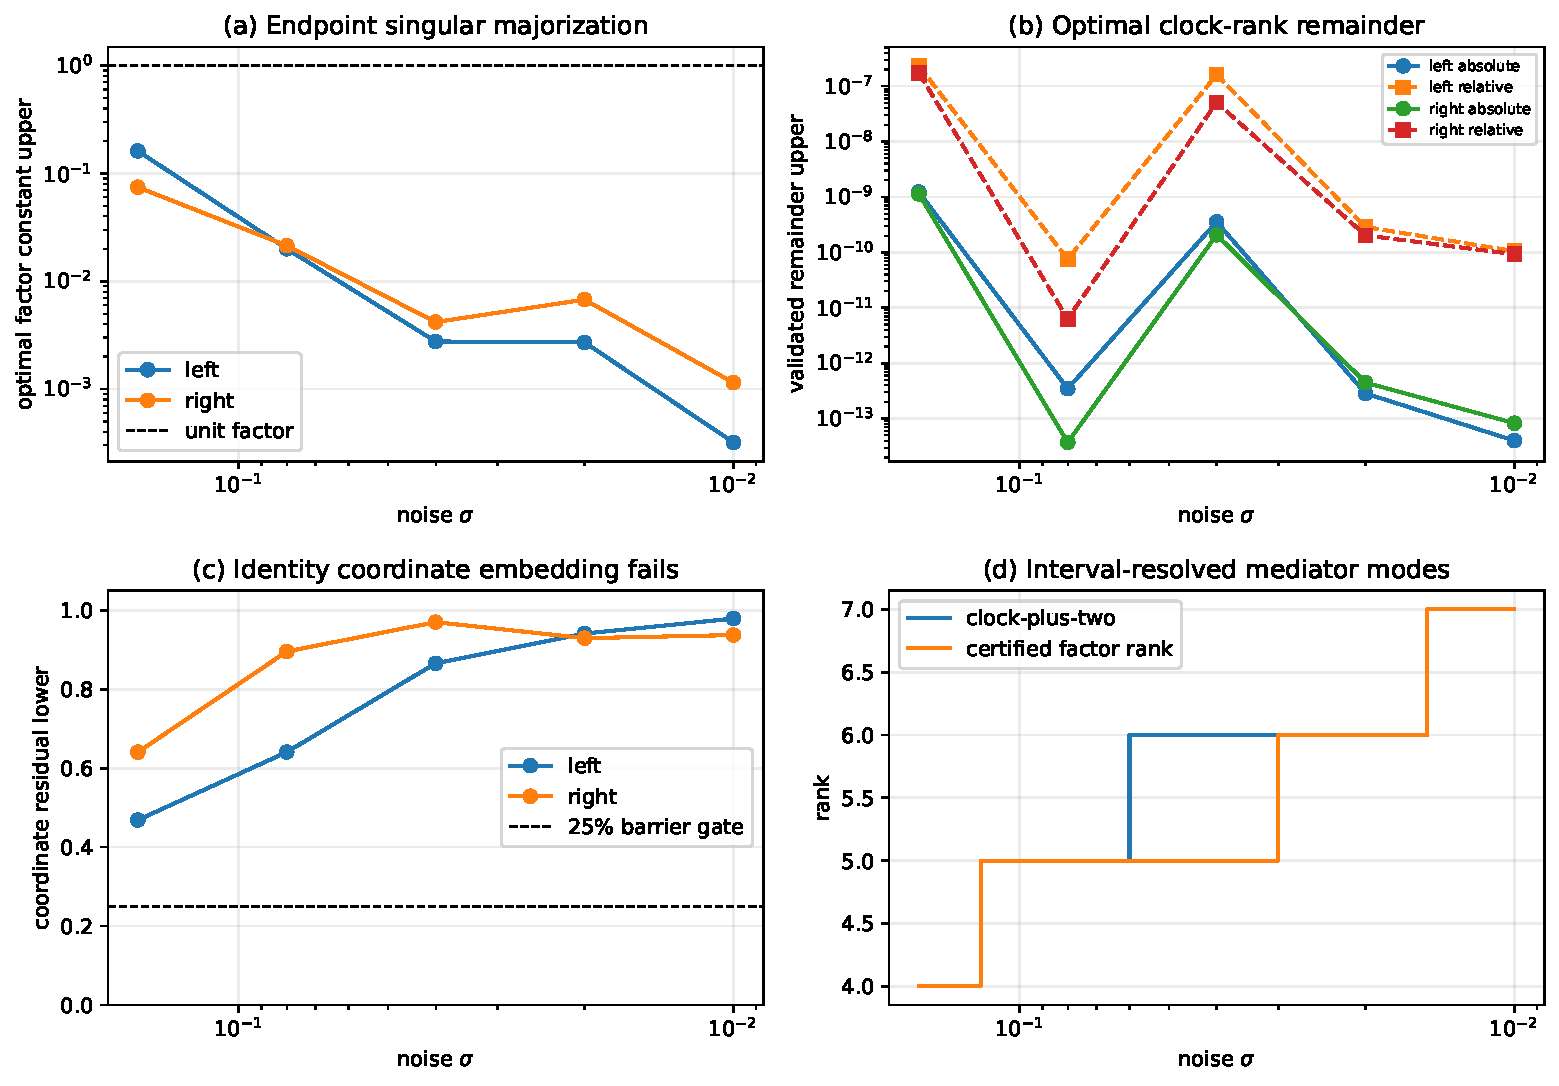
\includegraphics[width=\textwidth]{figures/optimal_endpoint_singular_factorization.pdf}
\caption{Optimal factor constants, SVD remainders, failure of direct
coordinate matching, and interval-resolved endpoint ranks.}
\label{fig:factor}
\end{figure}

\section{Next gate and claim boundary}

RH-83 removes a potentially expensive and false obligation.  One need not
identify physical postblock singular vectors with endpoint row vectors.
Instead, the next theorem should prove the scalar majorization
\eqref{eq:majorization} and tail bound \eqref{eq:remainder} uniformly over the
dyadic family.  A natural route is to compare physical Gram eigenvalues with
the exact endpoint Gram kernel through min--max or Schur-complement bounds,
allowing nontrivial dynamical outer maps.

This paper proves the optimal factorization theorem and validates finite
singular majorization at five scales.  It does not prove all-level
majorization, uniform Stage A1, unconditional Stage A4, a relative A5
determinant, a self-adjoint Hilbert--Polya operator, a $T\log T$ law, a
prime-power trace formula, a zeta-zero identification, or the Riemann
Hypothesis.

\bibliographystyle{plainnat}
\bibliography{references}

\end{document}
